\documentclass{article}
\usepackage[UTF8]{ctex}
\renewcommand{\figurename}{Figure}
\usepackage{graphicx}
\usepackage{subcaption}
\usepackage{listings}
\usepackage{placeins}
\lstset{
  basicstyle=\ttfamily\small, 
  breaklines=true,             
  backgroundcolor=\color{black!5}, 
  keywordstyle=\color{blue},   
  stringstyle=\color{red},   
  commentstyle=\color{green!70!black}, 
  literate={_}{\_}{1}          
}
\title{SI100B Handwritten Number Recognition Project Report}
\author{魏玄霖~向伊婷~洪悦}
\date{January 2026}

\begin{document}

\maketitle
\noindent\textbf{Author Contributions:} \\
魏玄霖: Software development and algorithm optimization \\
向伊婷: Hardware integration and functional testing \\
洪悦: Software development and functional testing
\section{Course design content}
In this course project, we designed and implemented a handwritten digit recognition system based on the K-Nearest Neighbors (KNN) algorithm, which was later replaced by a Support Vector Machine (SVM), combined with hardware output using a Raspberry Pi and a digital tube.
\subsection{Software design description}
\subsubsection{Creating training dataset}
We first imported a training photoset of 500 samples of each number from 0 to 9. Each image was converted from color to grayscale and then cropped into 20×20 pixel matrices, with one digit per matrix. This dataset trains the program to recognize what each number should look like.
\subsubsection{Image preprocessing, segmentation and reorganization}
The first step of the project was image preprocessing. The original color image captured by the camera was grayscaled and then binarized into a black-and-white image so the handwritten digits could be clearly distinguished from the background. This step reduced noise and simplified later processing. The key parameter in this step is the threshold: higher values cause more pixels to be converted to white.

Next, we segmented the binarized image. By analyzing the changes between black and white pixels along both the vertical and horizontal direction, we detected gaps between adjacent digits and split the image into several single-digit sub-images.

After segmentation, each digit image was further processed and reorganized into a two-level nested list, where each row of pixels was stored as a sub-list. This multi-level list structure makes it easier to output each row of digits separately on the digital tube later.
\subsubsection{Number recognition}
We then used the pre-trained KNN or SVM classification model to predict the handwritten digits, and finally a two-level nested list of digits will be output, where each sublist represents one row.
\subsection{Hardware design description}
Finally, we built a hardware circuit using a Raspberry Pi connected to a seven-segment digital tube. A camera attached to the Raspberry Pi captures an image when a button is pressed. As shown in the wiring diagram below, each Raspberry Pi pin controls one segment of the display. To protect the LED, we used 3.3V instead of 5V.
\begin{figure}[htbp]
	\centering
	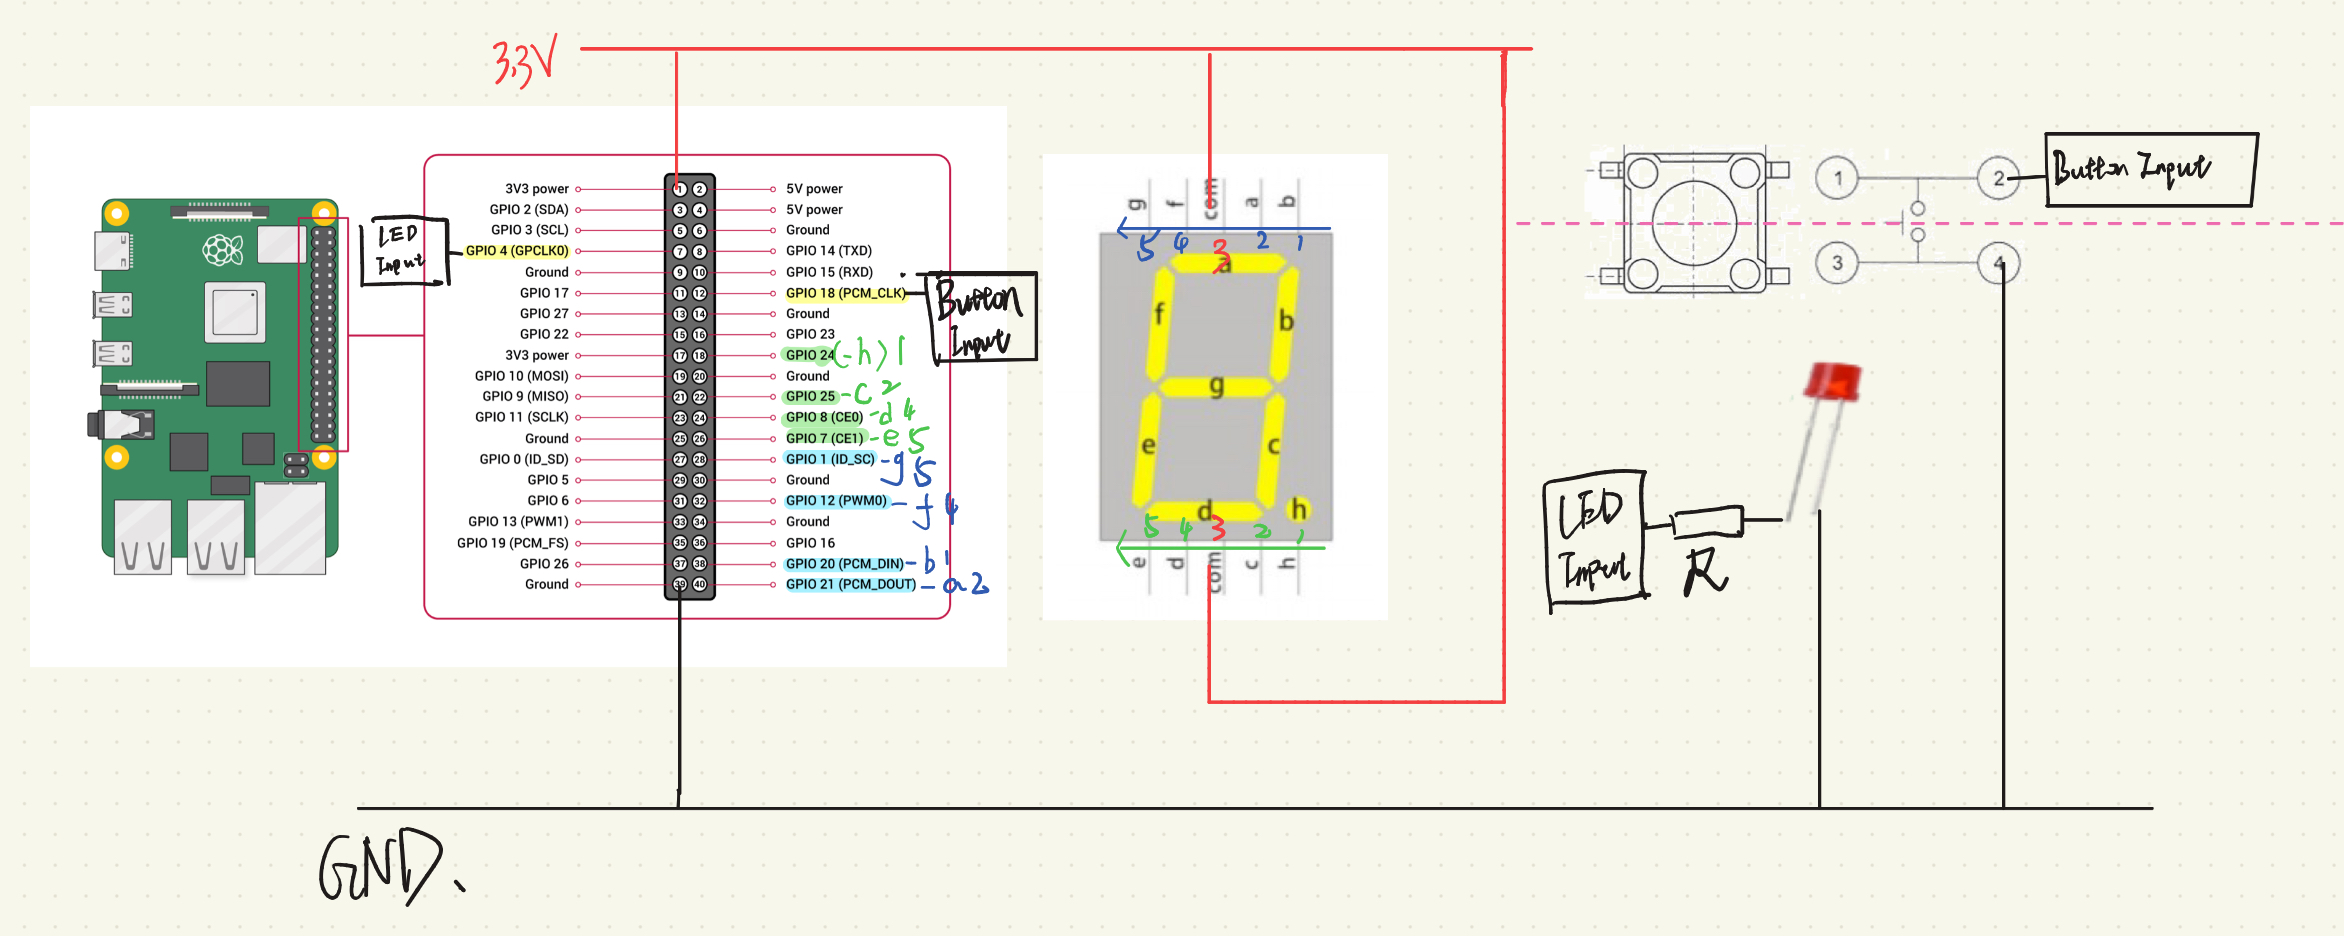
\includegraphics[width=0.85\textwidth]{wiring.jpeg}
	\caption{Wiring diagram}
\end{figure}
\begin{figure}[htbp]
	\centering
	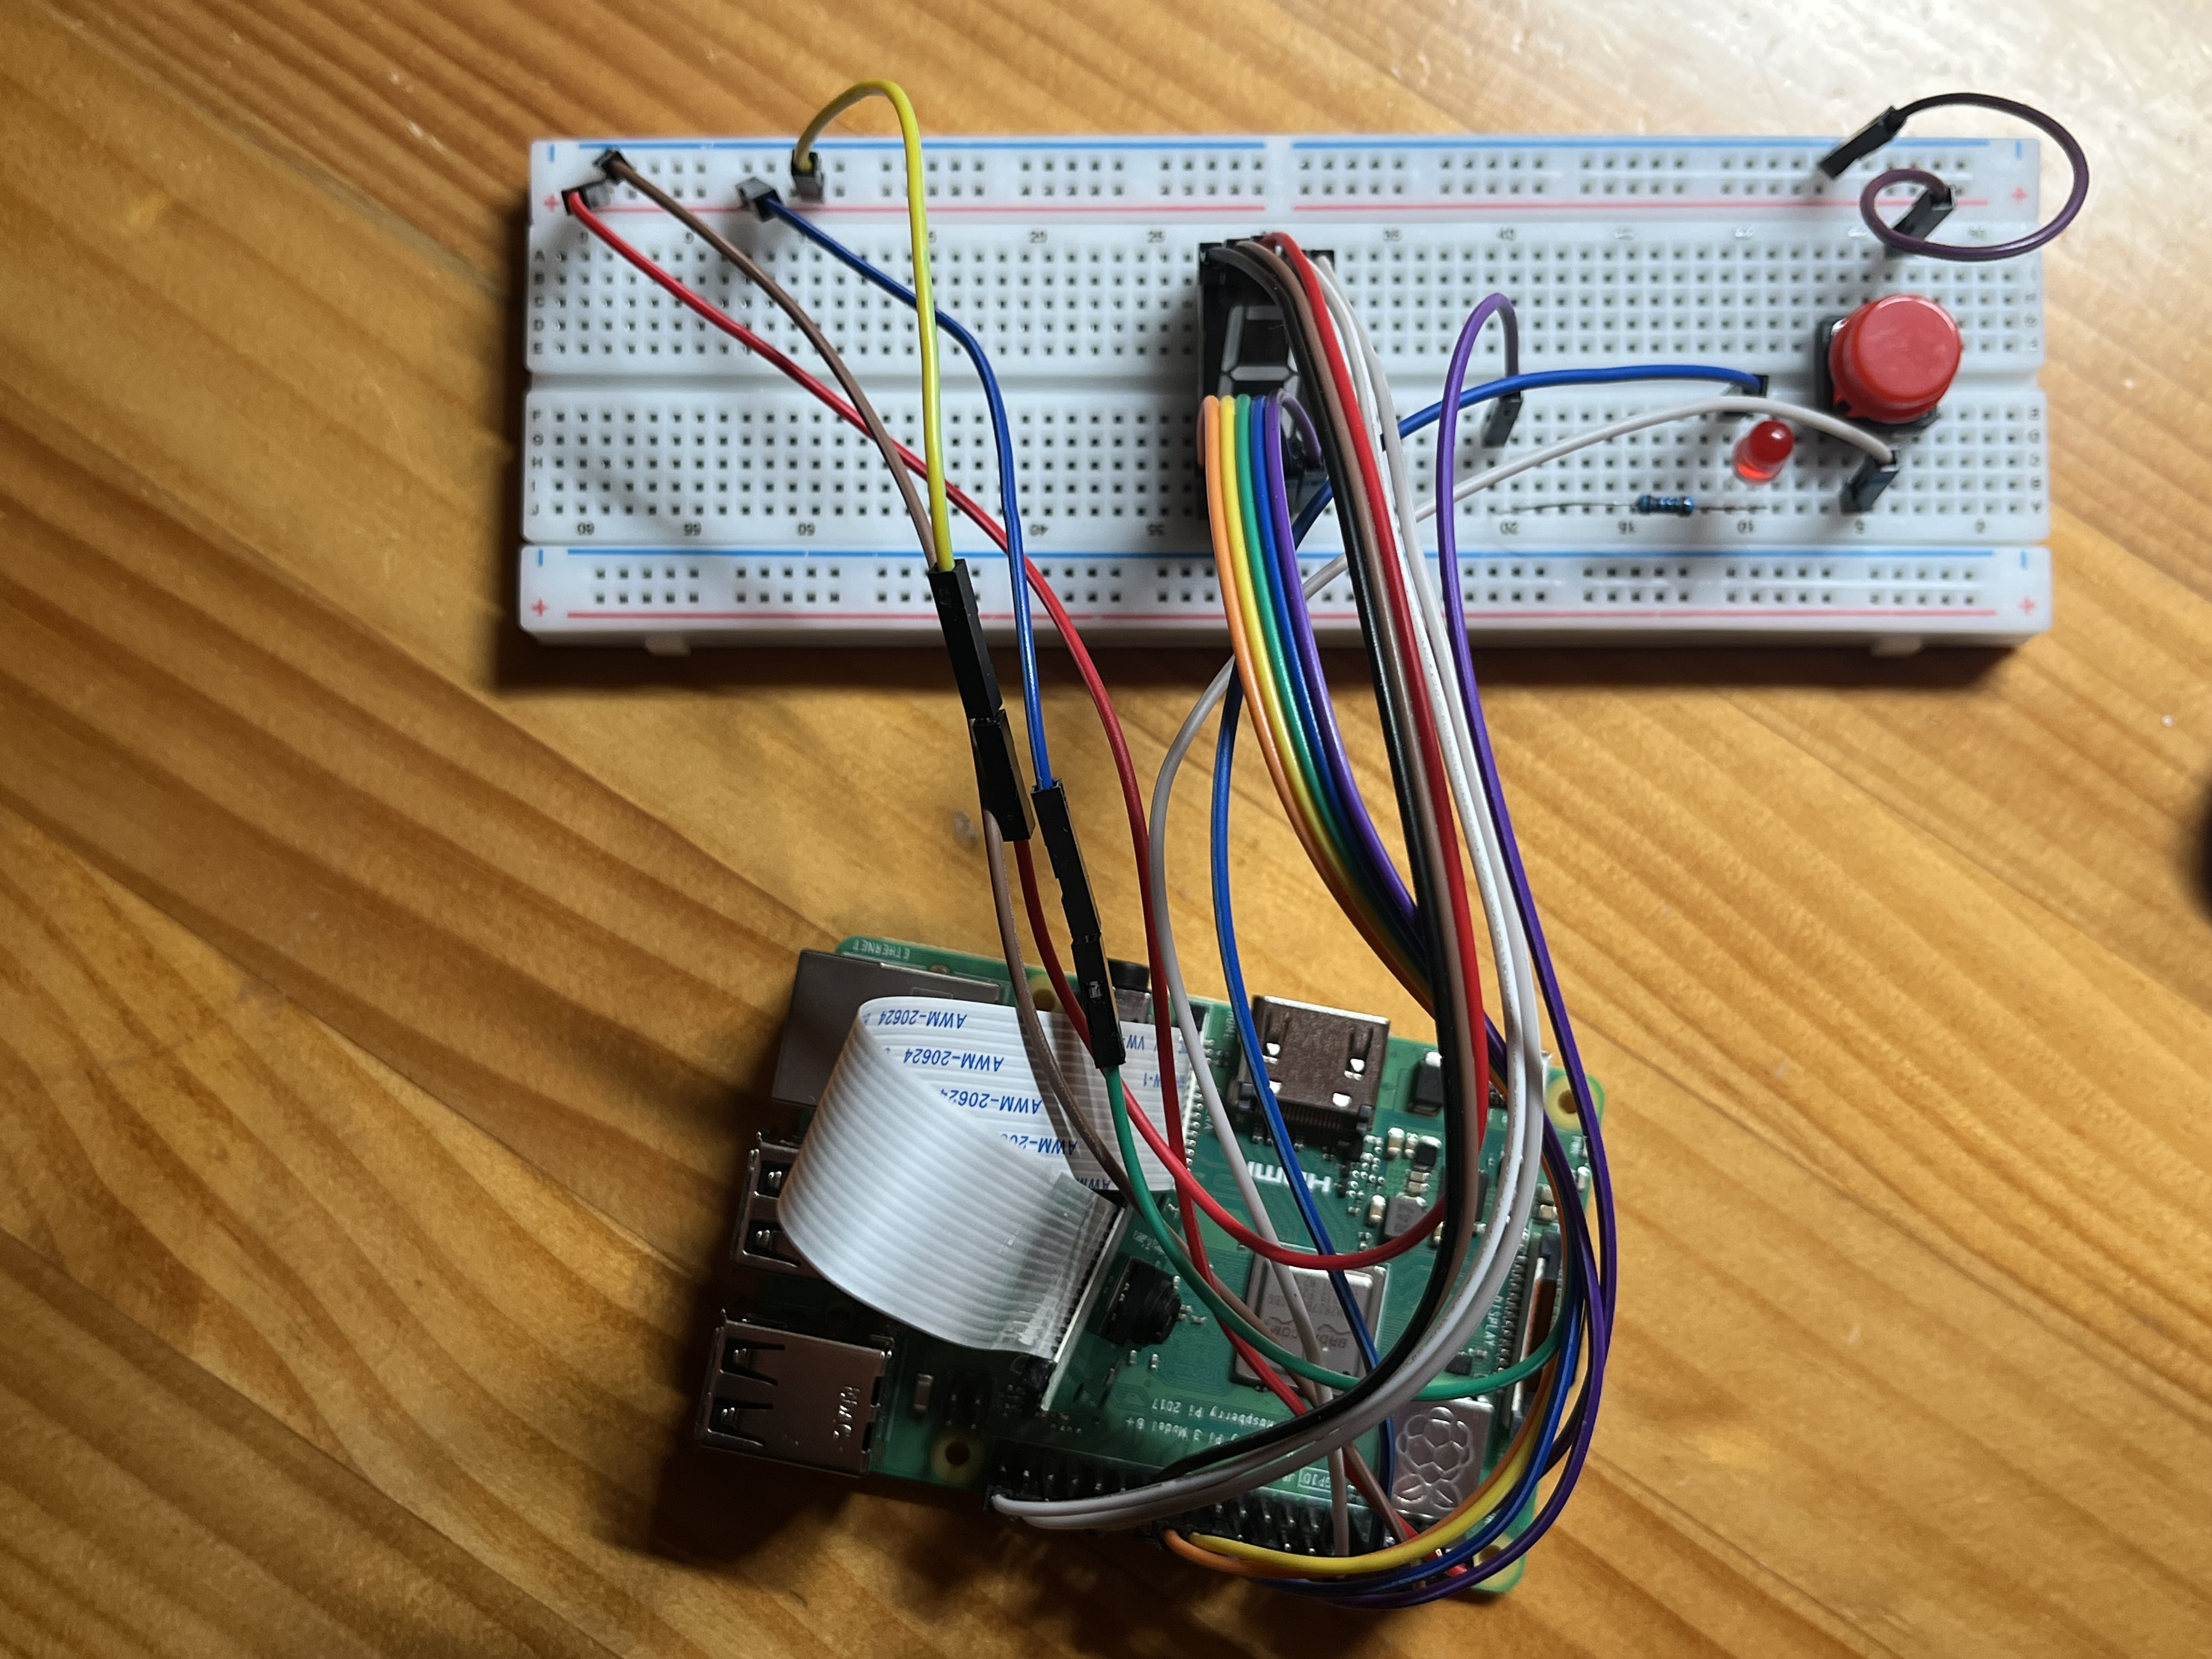
\includegraphics[width=0.85\textwidth]{setup.JPG}
	\caption{Hardware setup}
\end{figure}
\FloatBarrier
The recognition result produced by the KNN or SVM model was transmitted to the digital display, allowing the identified digit to be shown directly on the hardware device. The results are shown in sequence. Each number flashes for 1 second, and then switches to the next. Between lines there is a 2-second pause.
\section{Problems and Innovations}
\subsection{Improved image split function with a padding parameter} 
When we were preparing for the check on Lab 3, we found that the recognition accuracy was relatively low. Under the TA's instructions, we improved the image-splitting functions by adding paddings around the split image of each digit. In this way, we can adjust the padding size for different recognition tasks by modifying the parameters passed to the function, thereby achieving better recognition accuracy.

\subsection{Improved photo-taking process}
When following the example code on camera control from the lecture slides, we found that the preview window did not remain visible. Therefore, we transitioned to a non-blocking subprocess mechanism by setting the \texttt{-t} parameter duration from 5000 ms to 0 (infinite). By invoking \lstinline{preview_proc.terminate()} upon detecting a button press, we were able to maintain a continuous live preview before capturing the image. This ensures that the image framing and composition meet our expectations before the photo is taken.

\subsection{Optimized binarization function}
At first, we used the binarization method \lstinline{_, imgBin = cv2.threshold(imgGray, 180, 255, cv2.THRESH_BINARY_INV)}, as shown in the original Jupyter Notebook file. However, due to uneven illumination, unavoidable shadows often caused difficulties in finding a suitable binary threshold that could completely separate the digits from the background.

To solve this problem, we consulted several reference materials and applied some advanced OpenCV methods, including \lstinline{cv2.dilate}, \lstinline{cv2.medianBlur}, and \lstinline{cv2.absdiff}, to estimate the background illumination distribution and remove the background effect. As a result, we were able to obtain a high-quality binary image without manually adjusting the threshold parameter for photos taken under different lighting conditions.

\begin{figure}[htbp]
	\centering
	\begin{subfigure}{0.48\textwidth}
		\centering
		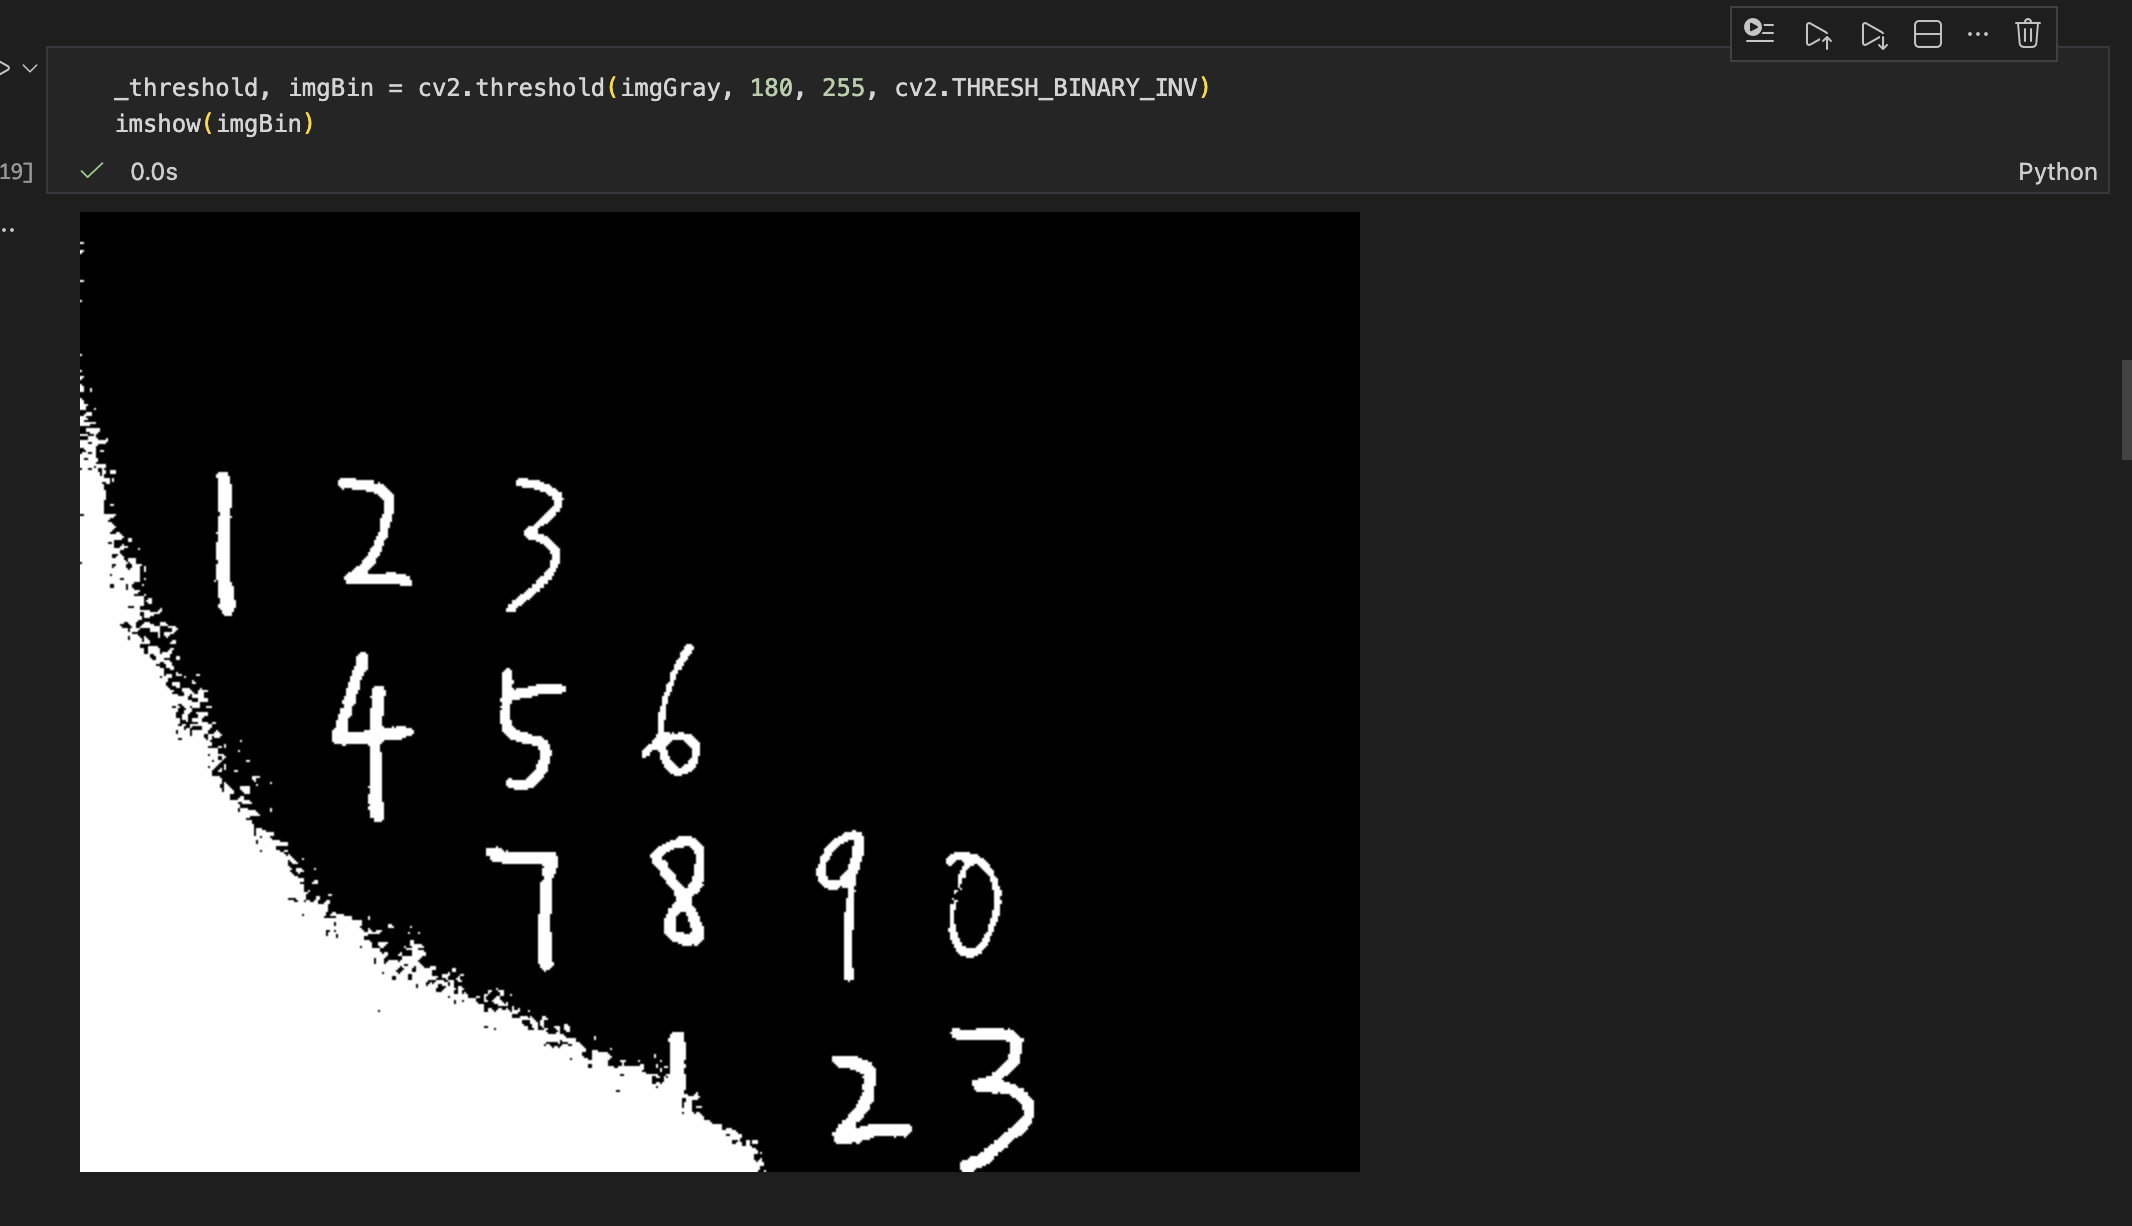
\includegraphics[width=\textwidth]{noise.png}
		\caption{}
	\end{subfigure}
	\hfill
	\begin{subfigure}{0.48\textwidth}
		\centering
		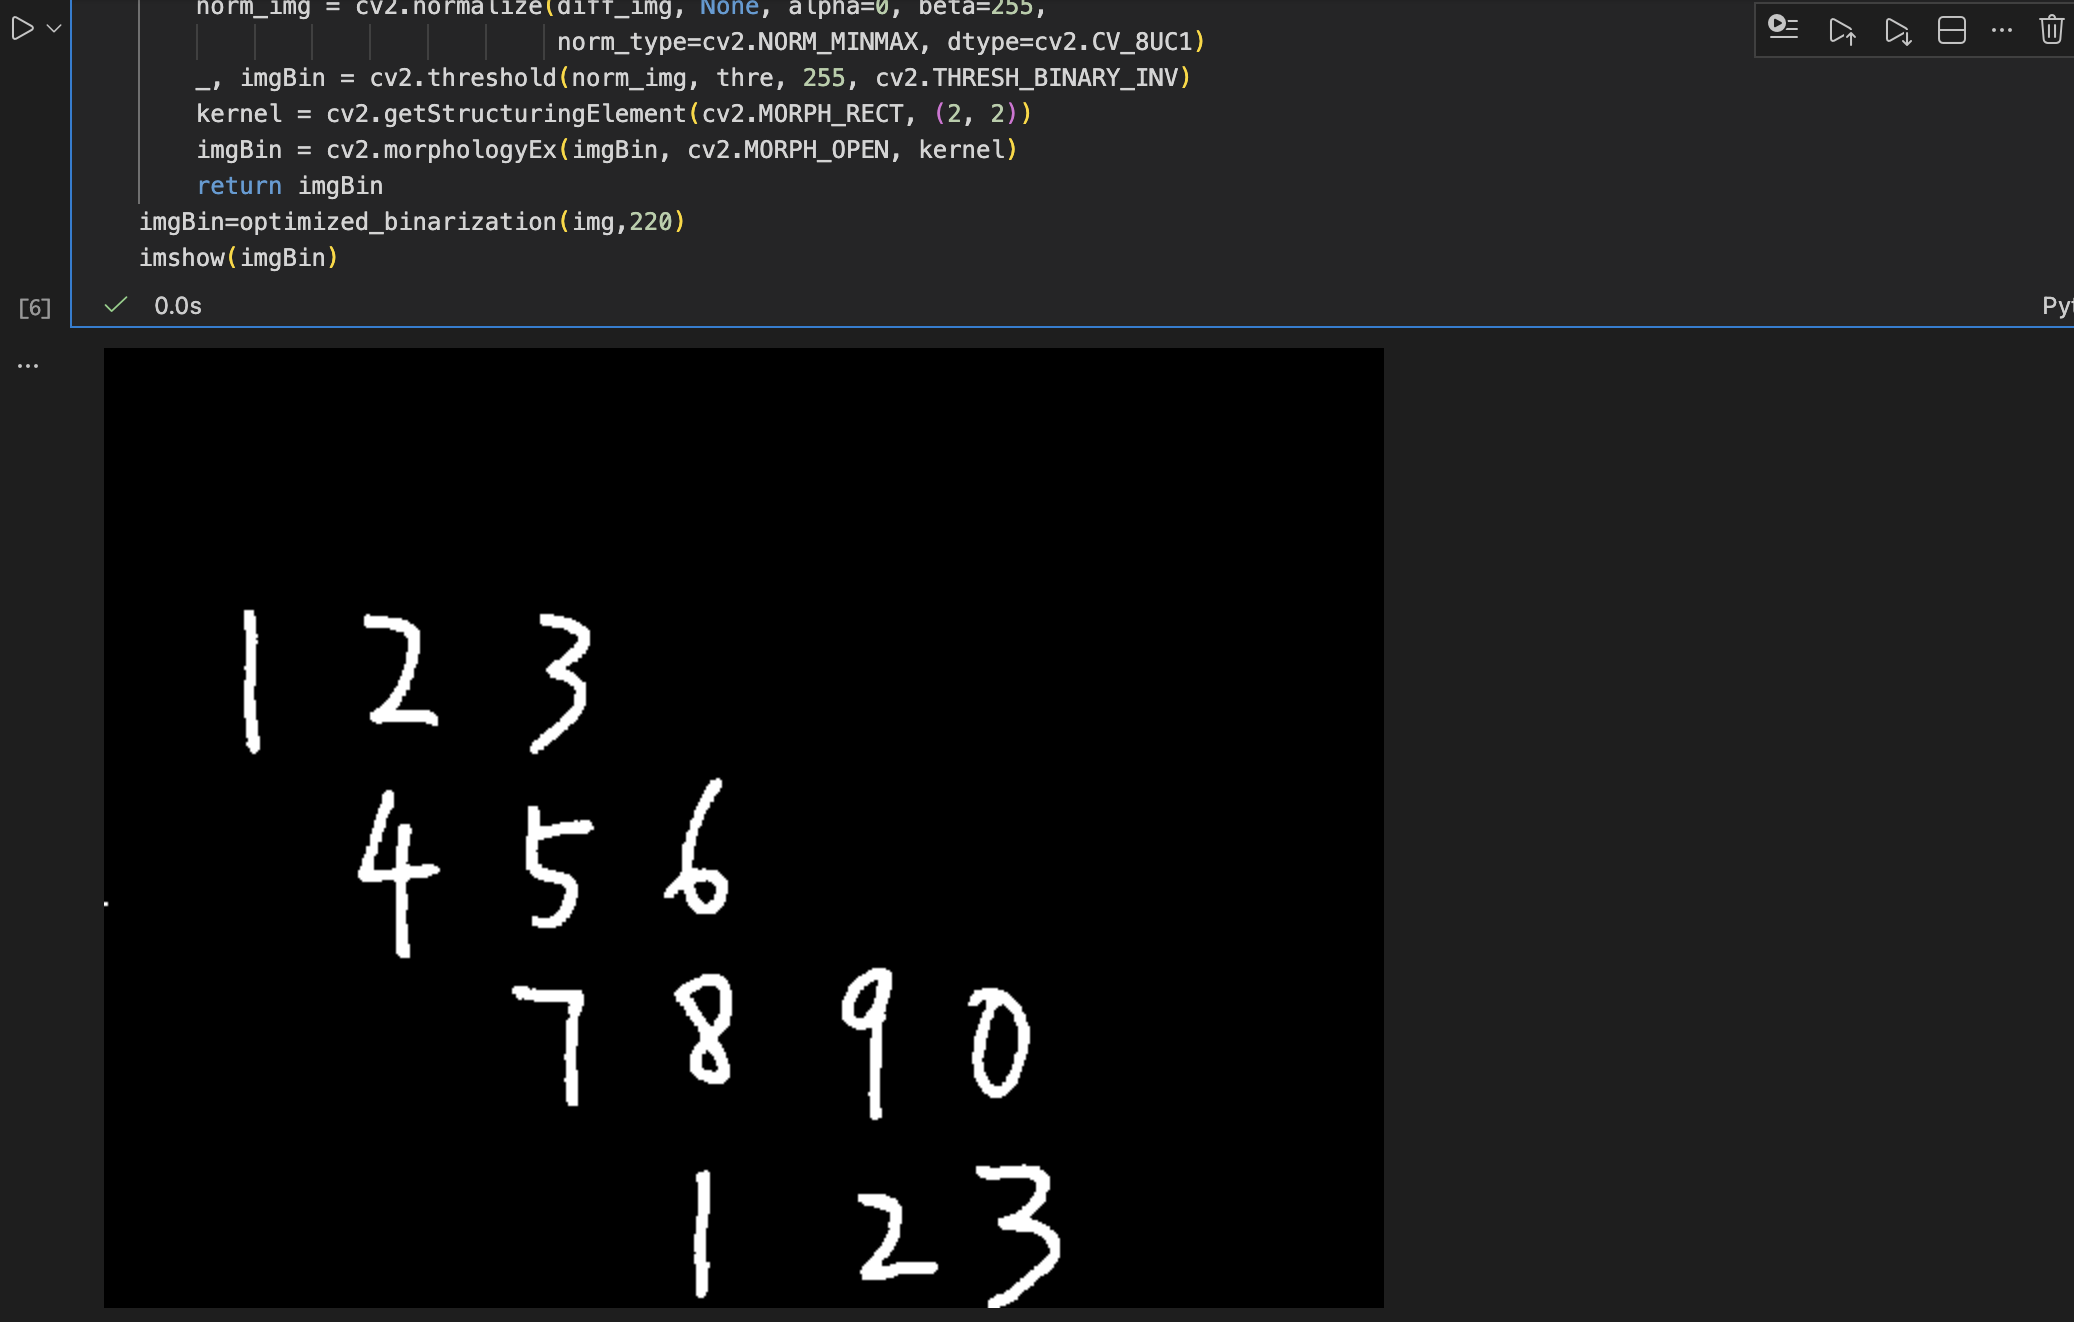
\includegraphics[width=\textwidth]{optbin.png}
		\caption{}
	\end{subfigure}
	\caption{Comparison of binary images between the original and optimized methods}
\end{figure}
\FloatBarrier
\subsection{Applying SVM algorithm instead of KNN}
In preparation for the final check, we attempted to apply the SVM algorithm instead of KNN to further improve recognition accuracy, and found that it performed effectively. We trained an SVM classifier with an RBF kernel, using $C = 12.5$ and $\Gamma = 0.02$.

\begin{figure}[htbp]
	\centering
	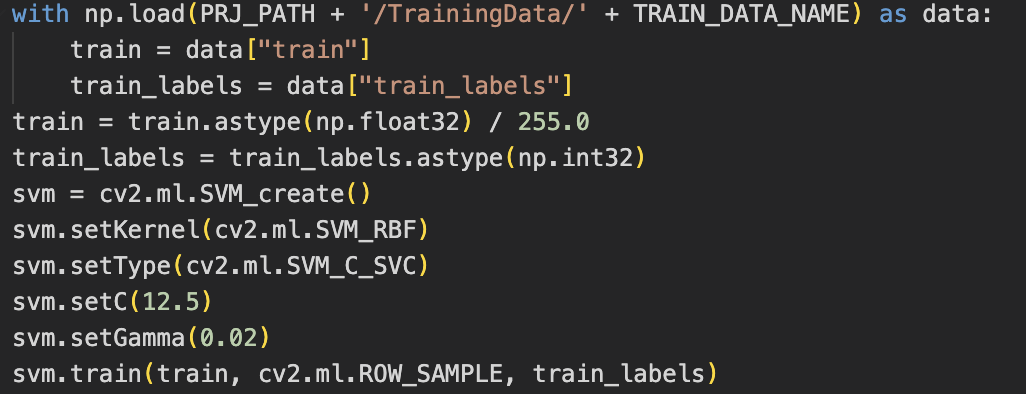
\includegraphics[width=0.85\textwidth]{SVM.png}
	\caption{SVM training code}
\end{figure}
\FloatBarrier

\subsection{Using wireless connectivity to facilitate team collaboration}
We connected the Raspberry Pi to a Wi-Fi hotspot provided by a mobile phone and ran Jupyter Notebook with the following parameters to bind it to both wired and wireless network addresses: \lstinline{jupyter notebook --ip=0.0.0.0 --no-browser --port=8888}. In this way, we were able to access the Jupyter Notebook webpage on multiple devices simultaneously, which greatly improved our team collaboration efficiency.

\subsection{Using Git and Github}
We used Git to host project files on GitHub, which provided a reliable way to better manage version control and team collaboration.
\begin{figure}[htbp]
	\centering
	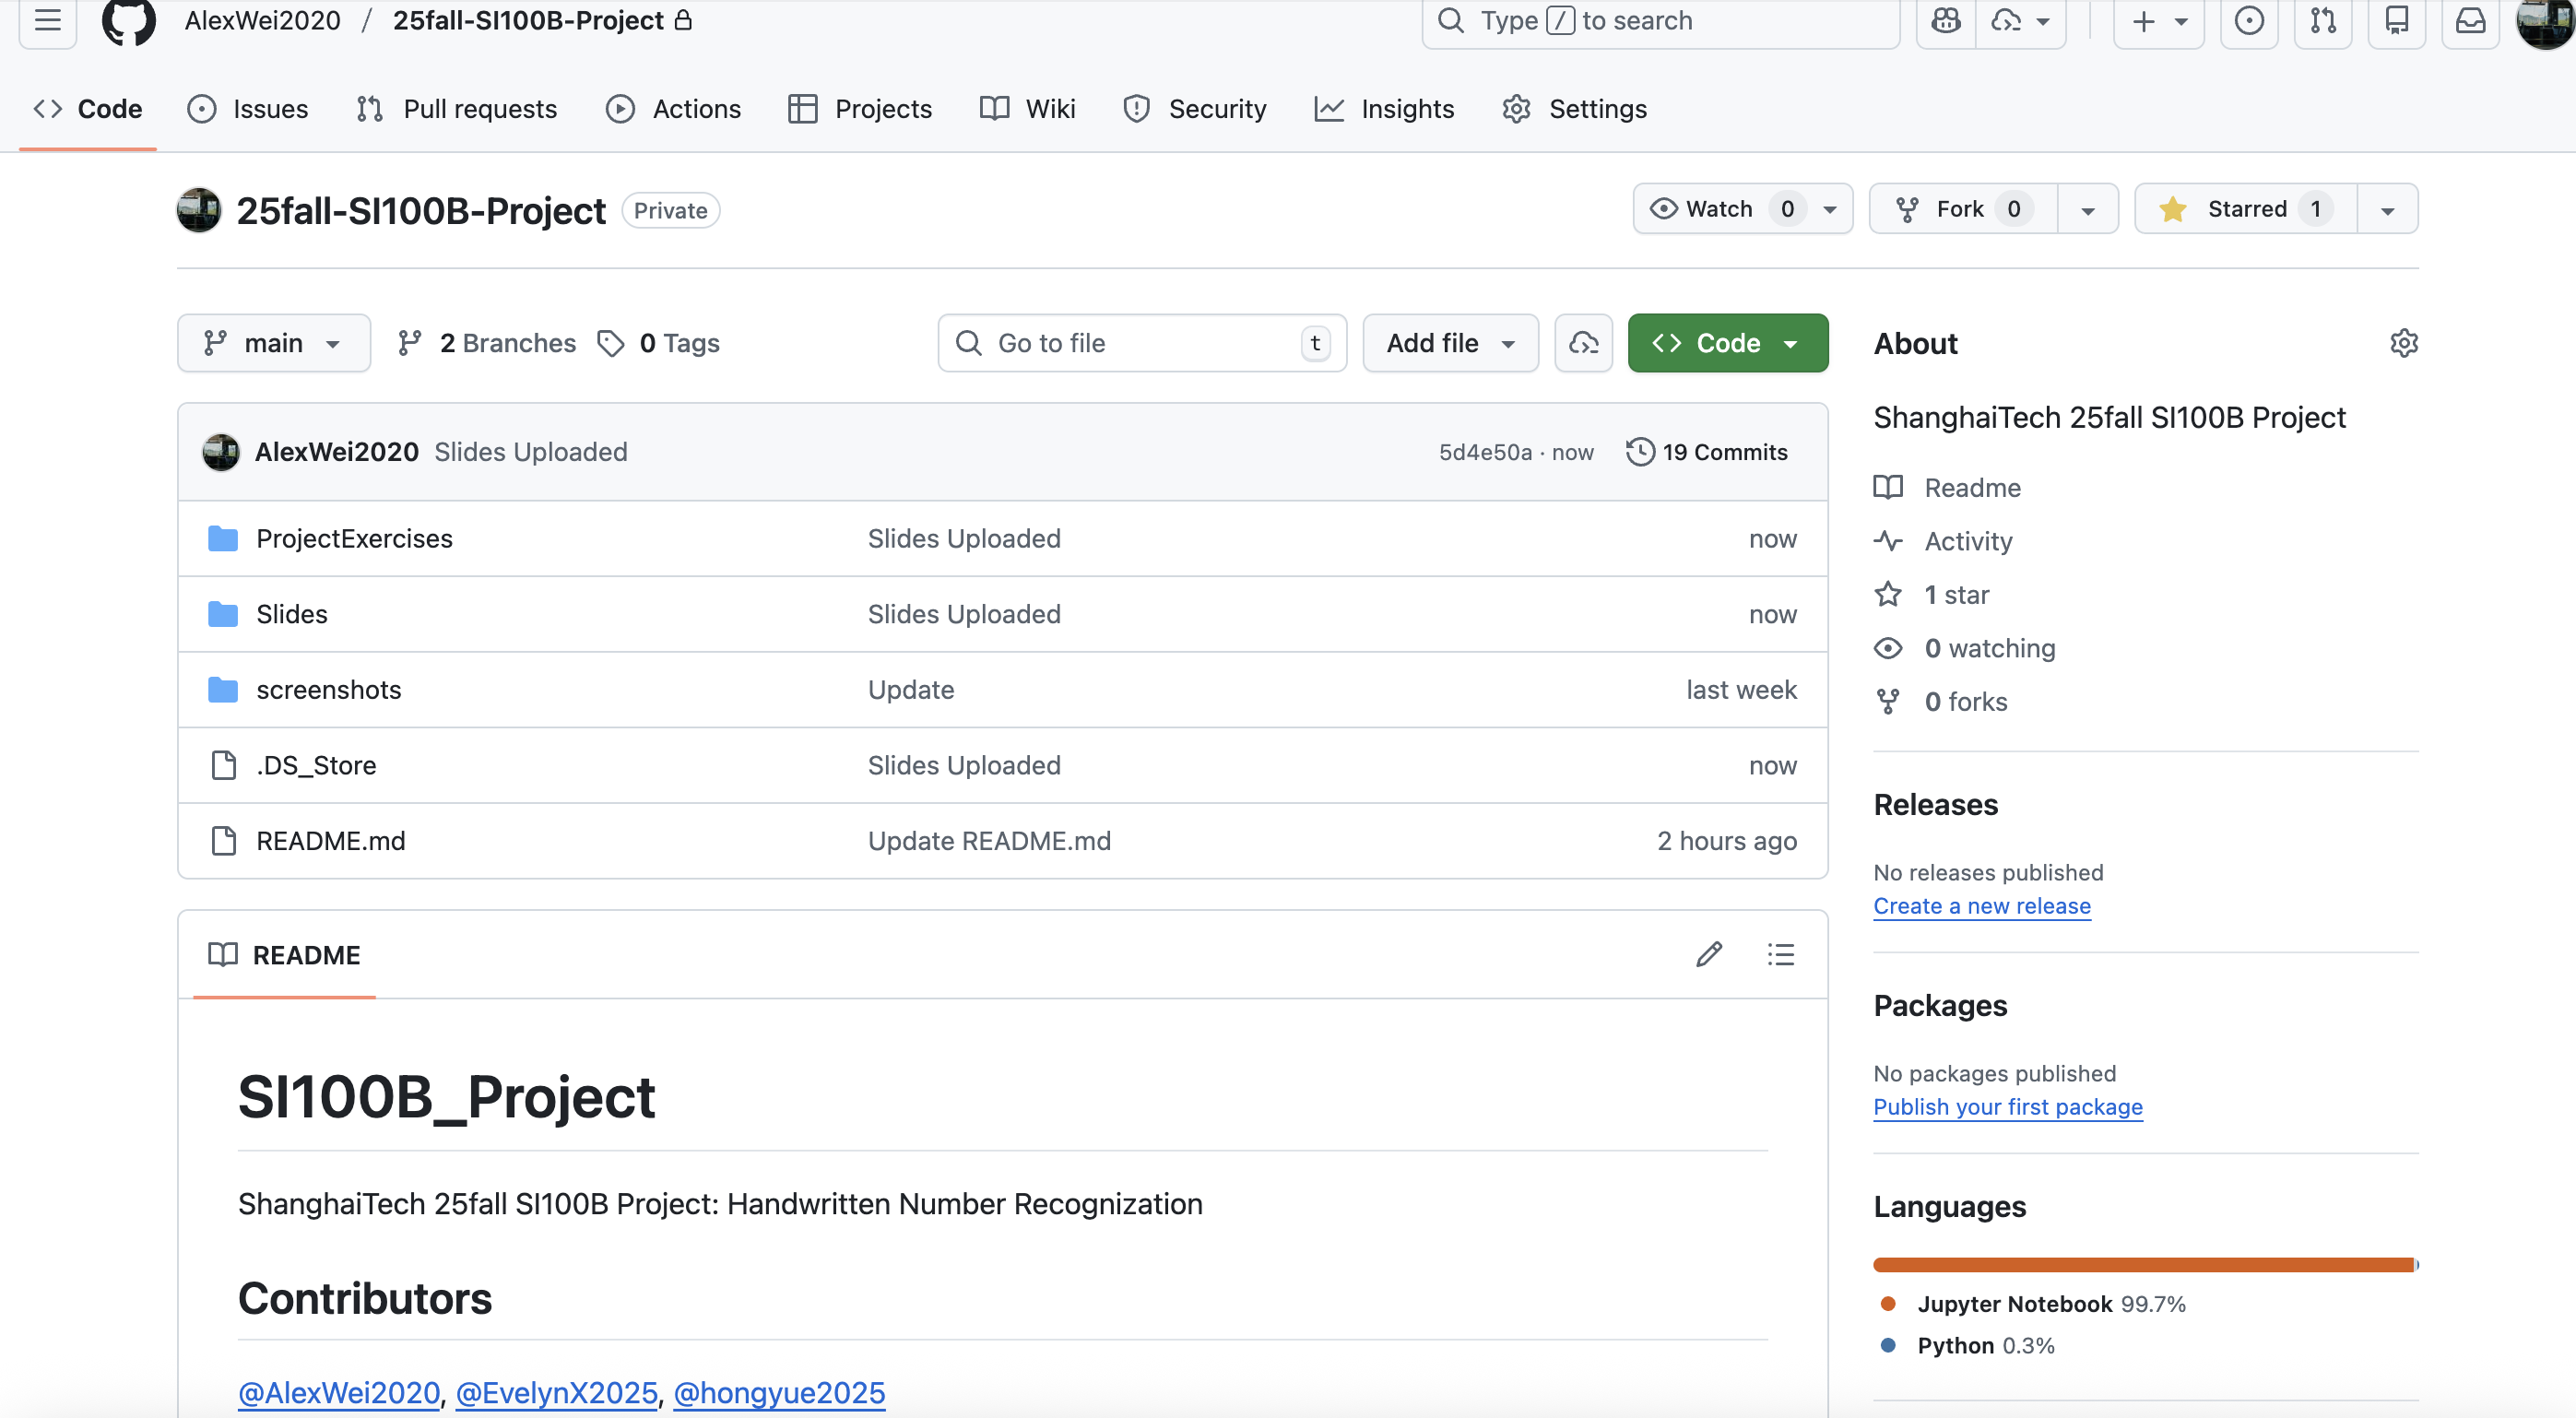
\includegraphics[width=0.85\textwidth]{github.png}
	\caption{Our github repository homepage}
\end{figure}
\FloatBarrier

\section{Final check demonstration}
\begin{figure}[htbp]
	\centering
	\begin{subfigure}{0.48\textwidth}
		\centering
		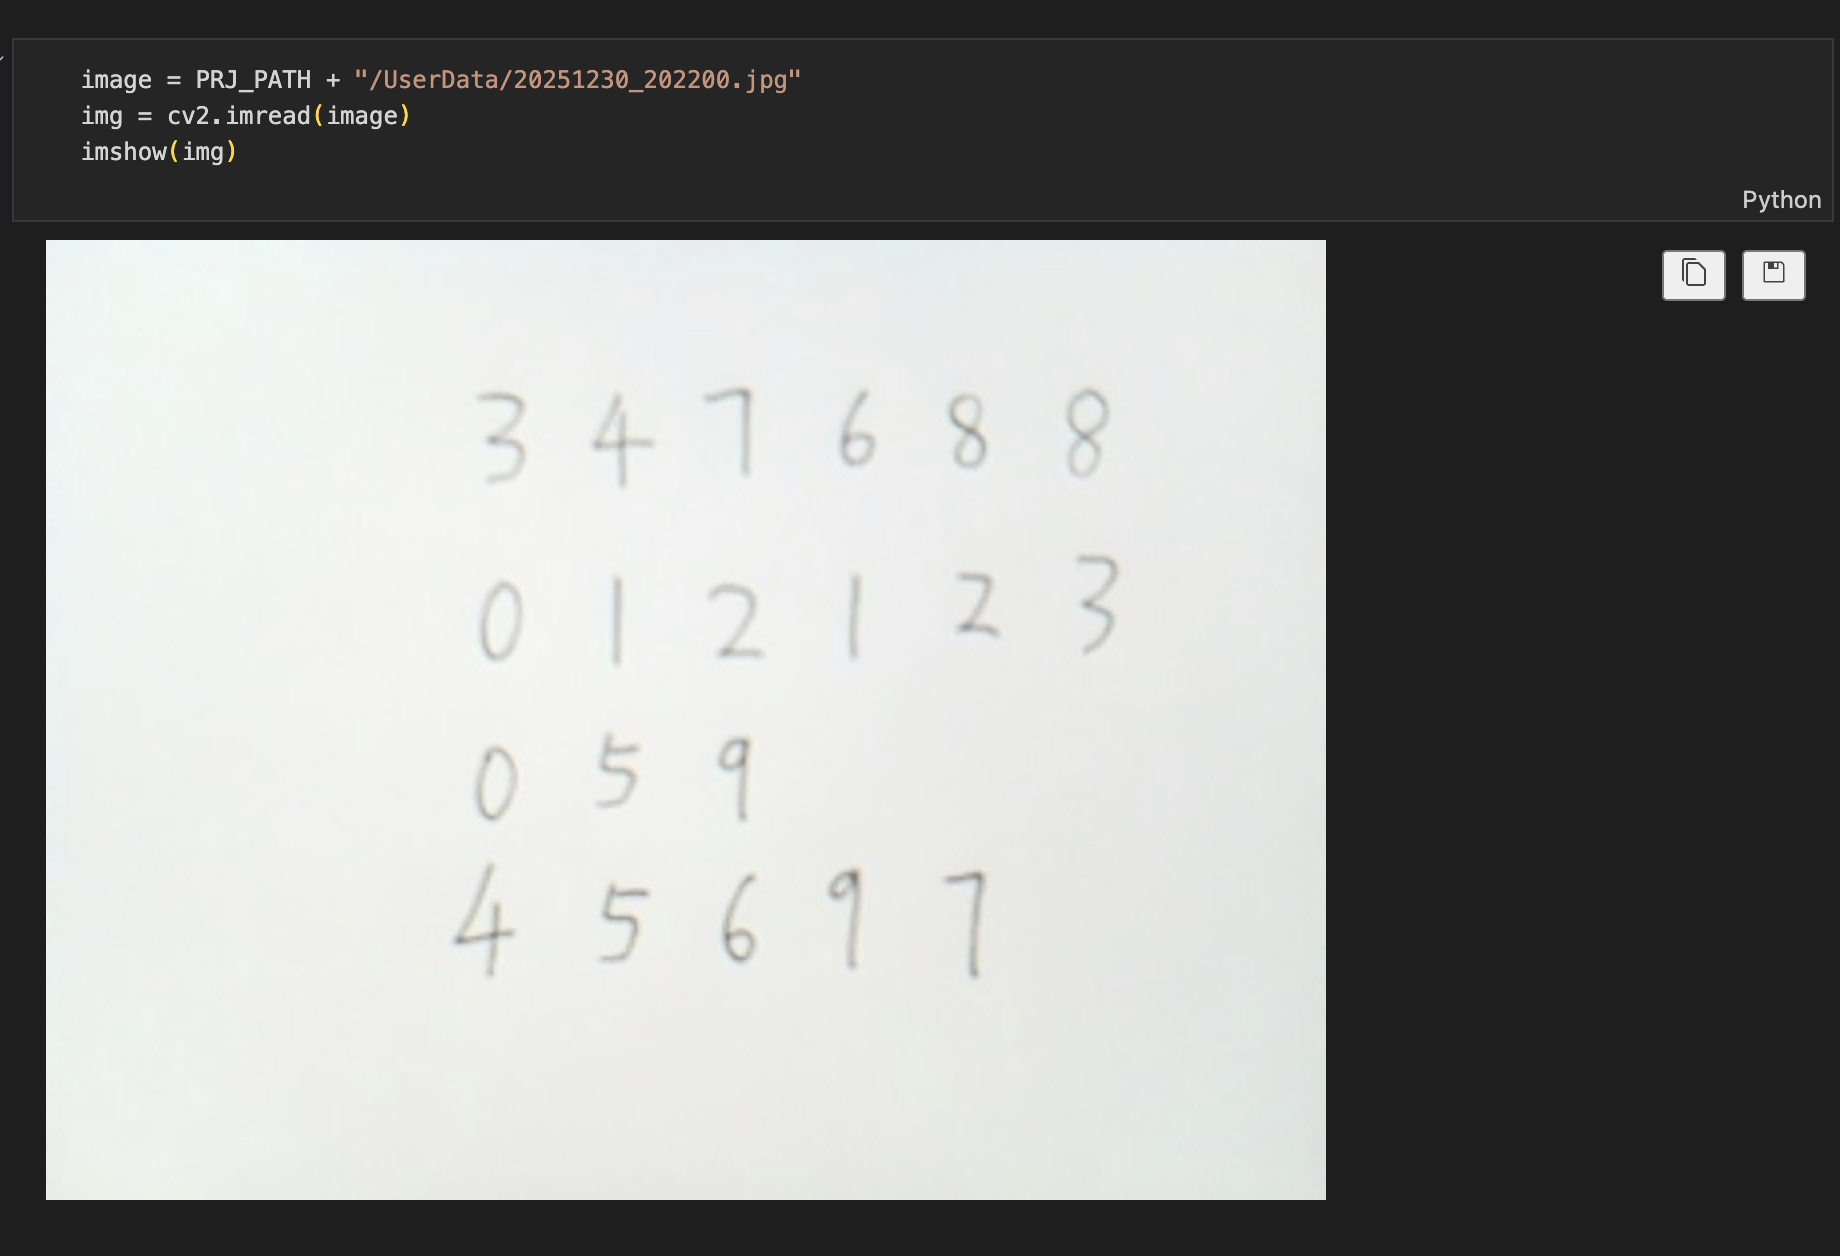
\includegraphics[width=\textwidth]{colorpic.png}
		\caption{}
	\end{subfigure}
	\hfill
	\begin{subfigure}{0.48\textwidth}
		\centering
		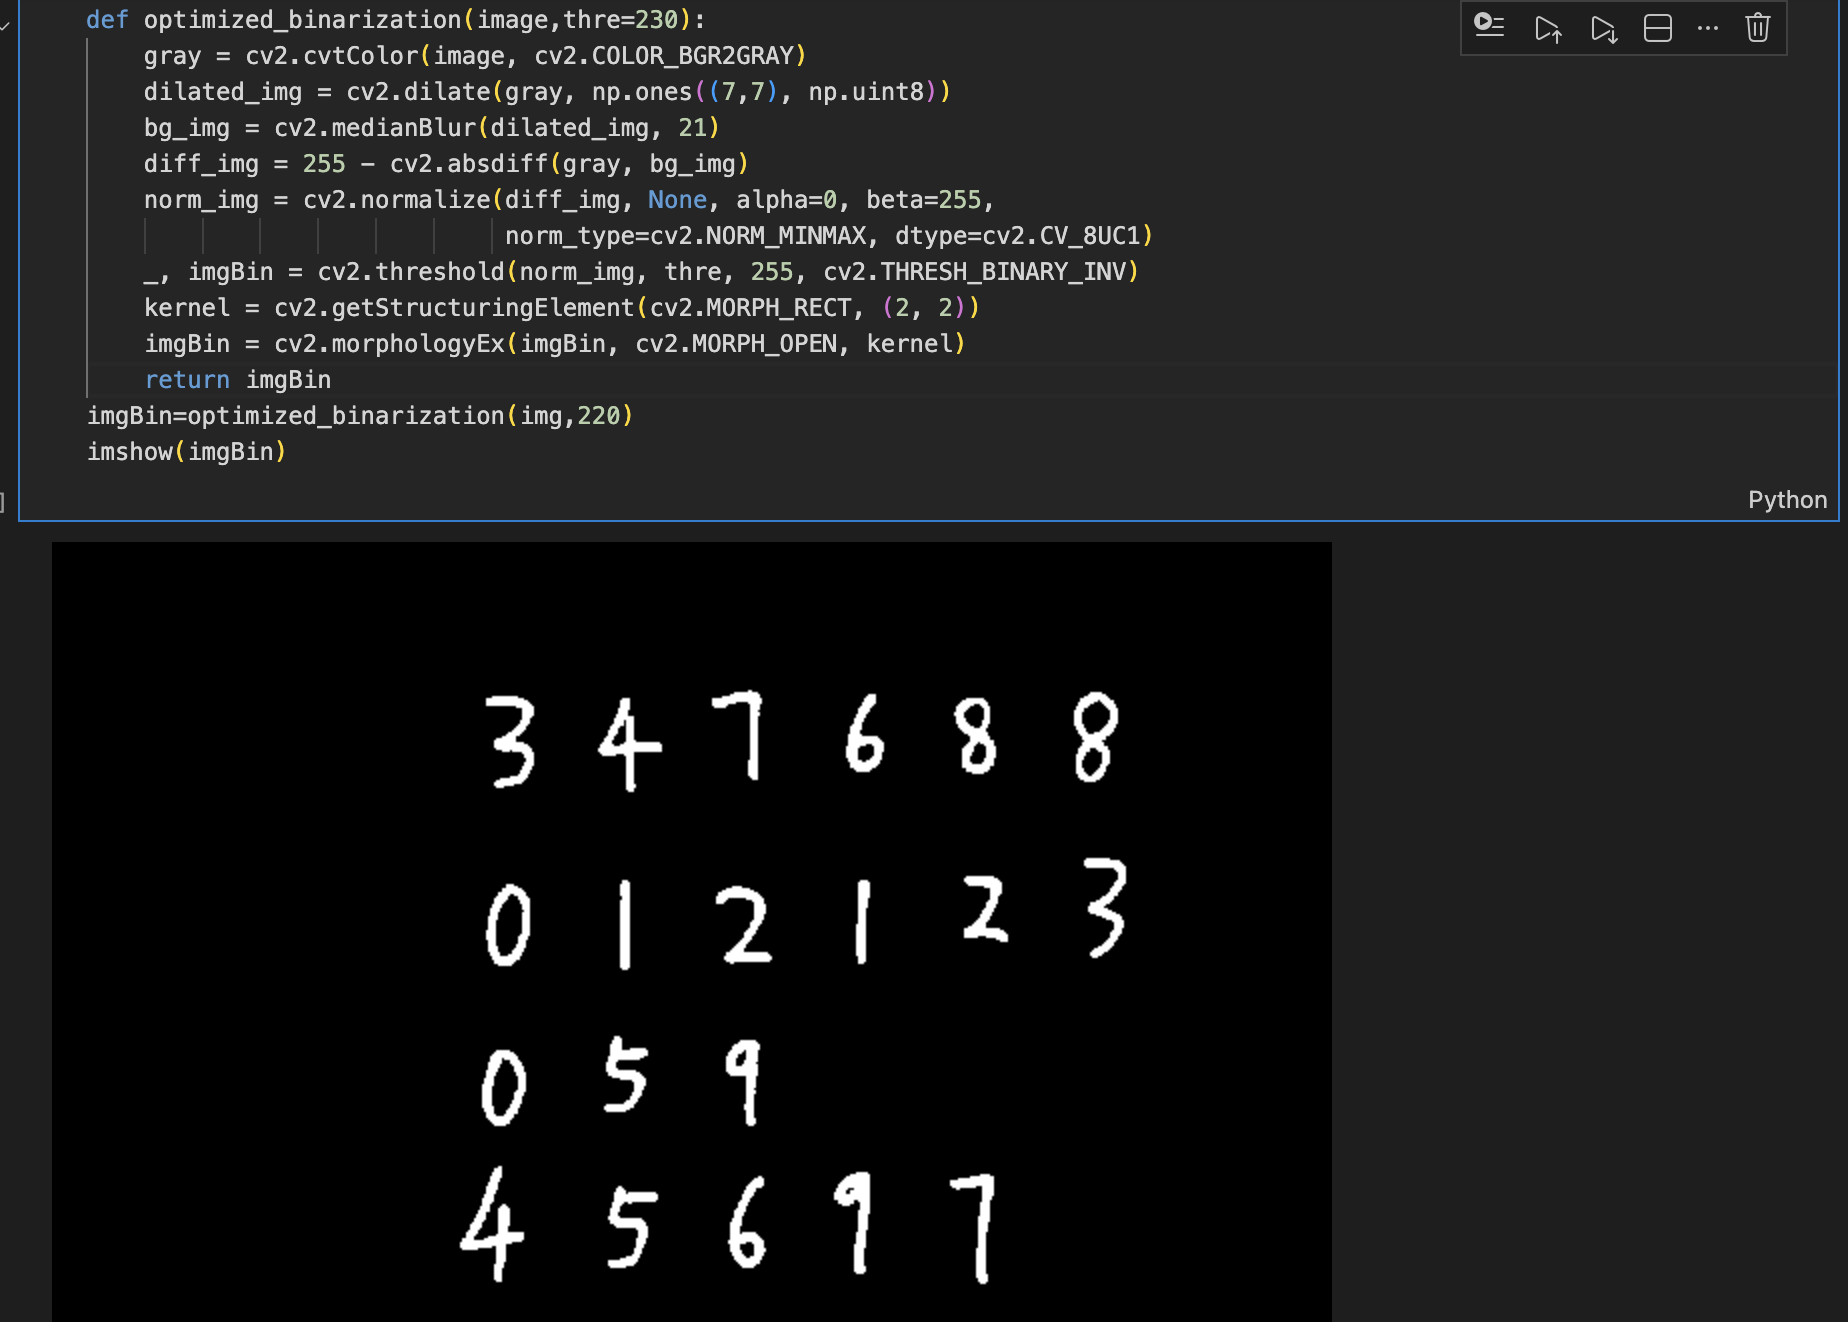
\includegraphics[width=\textwidth]{binpic.png}
		\caption{}
	\end{subfigure}
	\caption{Color image and binary image}
\end{figure}
\FloatBarrier
As shown in the figure below, 17 out of 20 numbers were correctly recognized during the final check.
\begin{figure}[htbp]
	\centering
	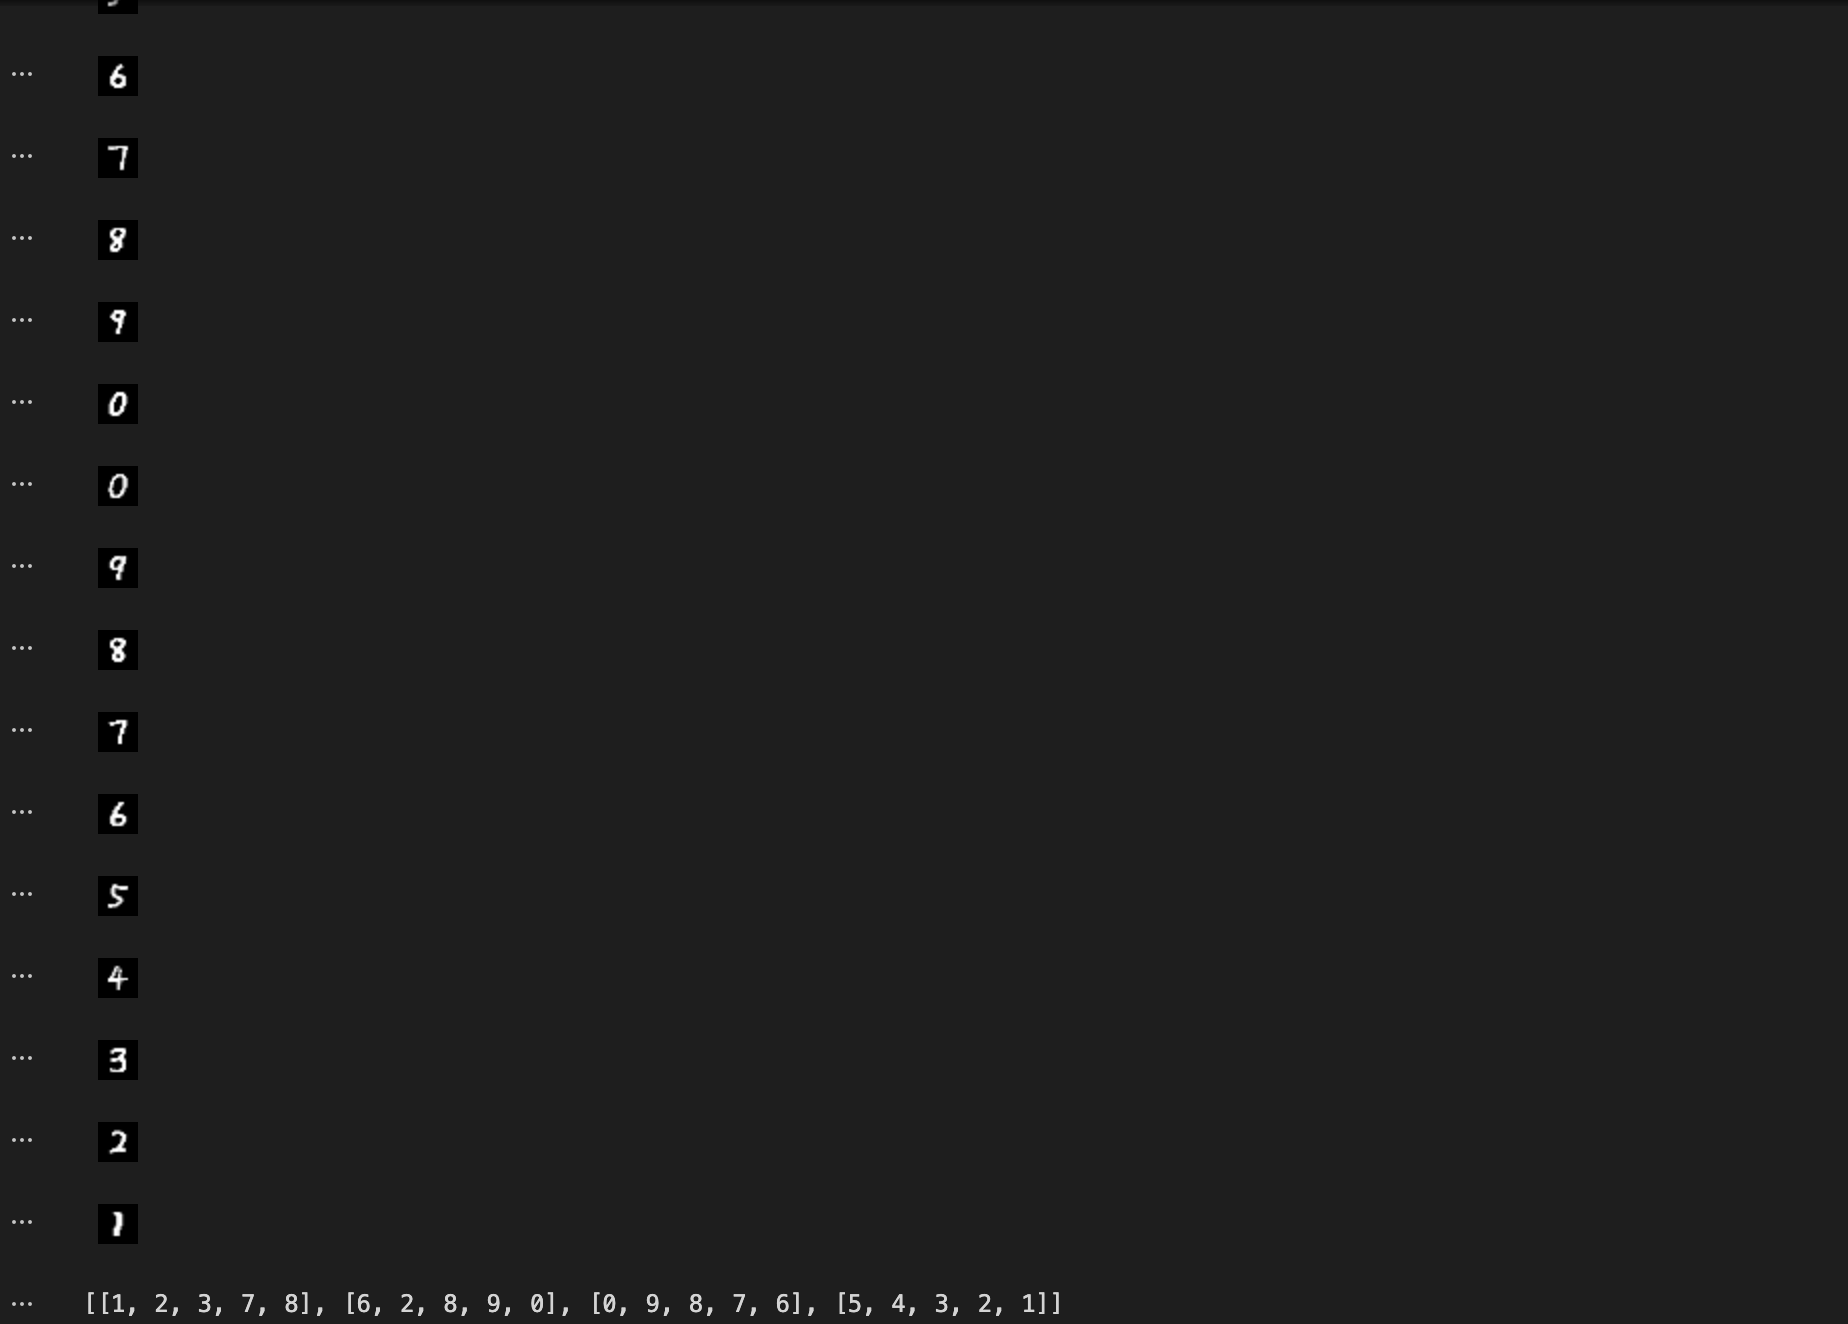
\includegraphics[width=0.85\textwidth]{result.png}
	\caption{Number recognition result}
\end{figure}
\FloatBarrier
\section{Personal reflection and thoughts}
Through this project, We gained a deeper understanding of how theoretical knowledge can be applied to real-world problems. Previously, machine learning algorithms such as KNN felt abstract, but implementing the entire pipeline—from image processing to model training and hardware output—made the concepts much clearer.

We also realized the importance of system-level thinking. A small issue in image preprocessing could significantly affect the final recognition result, which taught us that each step in a pipeline is closely connected. Moreover, combining software algorithms with hardware implementation was challenging but rewarding, as it required careful debugging and coordination.

Overall, this project strengthened our interest in information processing and intelligent systems. It helped us build confidence in tackling interdisciplinary problems and motivated us to explore more advanced applications of machine learning in the future.

\end{document}

